\documentclass[../main.tex]{subfiles}

\begin{document}
    \section{Differentiable Manifolds}
    \subsection{Definition}
    \subsubsection{Coordinate Charts}
    \begin{definition}[Coordinate Charts]\label{def:coordinate-charts}
        An \(m\)-dimensional, \(m \neq \infty\) coordinate chart on a topological 
        space \(\manifold\) is a pair 
        \[
        (U, \phi)
        \begin{cases}
            U \subseteq \manifold[M], U~\text{open}\\
            \phi : U \to \mathbb{R}^{m}, \phi~\text{homeomorphism}
        \end{cases}
        \]
        \begin{center}
            \begin{tikzpicture}
    \begin{scope}
        \irrshape{2}{0.1}{6};
    \end{scope}
    \node at (-1, 1) {$\manifold[M]$};
    \begin{scope}[xshift=0.5cm, yshift=-0.5cm]
        \irrshape{1}{0.05}{5}[dashed];
    \end{scope}
    \node at (1, -1) {$U$};
    \begin{scope}[xshift=4cm, yshift=-3cm]
        \begin{scope}[xshift=0.5cm, yshift=0.5cm]
            \irrshape{1}{0.2}{5}[dashed];
        \end{scope}
        \draw[->] (0, -0.5) -- (0, 2) node[above] {$\mathbb{R}^m$};
        \draw[->] (-0.5, 0) -- (2, 0);
    \end{scope}
    \draw[->] (1, -0.5) to [out=-10, in=105] node [auto] {$\phi$} (3.8, -2.5) ;
\end{tikzpicture}
        \end{center}
    \end{definition}
    \begin{remark}
        If \(U=\manifold[M]\), then we say the coordinate chart \(\phi\) is 
        globally defined; if not, then it is locally defined. Few manifolds 
        have globally defined property.
    \end{remark}
    \begin{remark}
        The basic method of studying manifolds is to analyze it in the familiar 
        Euclidean space via coordinate charts.
    \end{remark}
    \newpage
    \begin{definition}[Overlap Function]\label{def:overlap-function}
        Let \((U_1, \phi_1), (U_2, \phi_2)\) be a pair of \(m\)-dimensional 
        coordinate charts with \(U_1 \cap U_2 \neq \varnothing\). Then the 
        overlap function is defined as 
        \[
        \phi_2\circ\phi_1 ^{-1} : \phi_1(U_1 \cap U_2) \subseteq \mathbb{R}^m 
        \to \phi_2(U_1 \cap U_2) \subseteq \mathbb{R}^m.
        \]
        \begin{center}
            \begin{tikzpicture}
    \irrshape{2.5}{0.5}{6};
    \node at (-1, 1.5) {$\manifold[M]$};
    \begin{scope}[xshift=0.5cm]
        \irrshape{1}{0.05}{5}[dashed];
    \end{scope}
    \node at (1, -1.3) {$U_1$};
    \begin{scope}[xshift=-0.5cm]
        \irrshape{1}{0.05}{5}[dashed];
    \end{scope}
    \node at (-1.3, -1) {$U_2$};
    \node at (0, 0) {$U_1 \cap U_2$};
    \begin{scope}[xshift=4cm, yshift=-3cm]
        \begin{scope}[xshift=0.5cm, yshift=0.5cm]
            \irrshape{1}{0.2}{5}[dashed];
        \end{scope}
        \draw[->] (0, -0.5) -- (0, 2) node[above] {$\mathbb{R}^m$};
        \draw[->] (-0.5, 0) -- (2, 0);
    \end{scope}
    \draw[<-] (1, -0.5) to [out=-10, in=105] node [auto] {$\phi_1 ^{-1}$} (3.8, -2.5) ;
    \begin{scope}[xshift=-4cm, yshift=-3cm]
        \begin{scope}[xshift=0.5cm, yshift=0.5cm]
            \irrshape{1}{0.2}{5}[dashed];
        \end{scope}
        \draw[->] (0, -0.5) -- (0, 2) node[above] {$\mathbb{R}^m$};
        \draw[->] (-0.5, 0) -- (2, 0);
    \end{scope}
    \draw[->] (-1, -0.5) to [out=190, in=75] node [auto] {$\phi_2$} (-3.8, -2.5);
    \draw[->] (3, -2.5) to [out=190, in=-10] 
        node [auto] {$\phi_2\circ\phi_1 ^{-1}$} (-2, -2.5);
\end{tikzpicture}
        \end{center}
    \end{definition}
    \begin{definition}[Atlas]\label{def:atlas}
        An \(m\)-dimensional atlas on \(\manifold[M]\) is a family of 
        \(m\)-dimensional coordinate charts \((U_i, \phi_i), i \in I\) s.t. 
        \begin{enumerate}
            \item \(\manifold[M] = \bigcup_{i \in I}^{} U_i\).
            \item Each overlap function \(\phi_j \circ \phi_i ^{-1}, i, j \in I\) 
            is \(C ^{\infty}\).
        \end{enumerate}
    \end{definition}
    \begin{definition}[Differentiable Manifolds]\label{def:differentiable-manifolds}
        An \(m\)-dimensional differentiable manifold is a topological space 
        \(\manifold[M]\) equipped with an atlas.
    \end{definition}
    \begin{remark}
        We didn't define a differentiable manifold by regulating the 
        differentiability of the coordinate charts themselves. That's because 
        differentiation is not defined on a manifold, so we need to rely on 
        Euclidean spaces.
    \end{remark}
    \newpage
    \subsection{Dimension of a Manifold}
    \begin{remark}
        Consider a manifold that consists of a rod attached to a disk. The dimension 
        is not same everywhere. We give a criterion on how to describe 
        such a scenario.
    \end{remark}
    \begin{theorem}[Invariance of Domain]\label{thm:invariance-domain}
        For all \(A, B \subseteq S^n\), if \(\exists~f : A \to B\) homeomorphic 
        and \(B \in \tau_{S^n}\), then \(A \in \tau_{S^n}\) too.
    \end{theorem}
    \begin{remark}
        \cref{thm:invariance-domain} is an early theorem in algebraic topology.
    \end{remark}
    \begin{corollary}[Dimension is Well-defined]\label{cor:manifold-dim-well-defined}
        Given \(U \in \tau_{\mathbb{R}^n}, U' \in \tau_{\mathbb{R}^{n'}}\), and if 
        \(\exists~f : U \to U'\) homeomorphic, then \(n = n'\).
    \end{corollary}
    \begin{proof}
        If \(n = n'\), it is trivially true. \par
        If \(n < n'\), embed \(\mathbb{R}^n\) to \(\mathbb{R}^{n'}\) by 
        \(f : \vec{x} \mapsto (\vec{x}, \vec{0})\). Via stereographic projection, 
        we can map homeomorphically
        \begin{align*}
            \phi &: U  \mapsto V \subseteq S^{n'}, \\
            \phi'&: U' \mapsto V' \subseteq S^{n'}.
        \end{align*}
        Since the compositions are also homeomorphic, we see \(V\) and \(V'\) are 
        homeomorphic. However, \(V'\) is not an open subset of \(\mathbb{R}^{n'}\) because 
        of the \(0\)'s, contradicting \cref{thm:invariance-domain}. 
        \textreferencemark
    \end{proof}
    \begin{remark}
        Since the definition of a differentiable manifold requires every overlap 
        function to be diffeomorphic, if \(U \cap U' \neq \varnothing\), their 
        dimensions must be equal via the above corollary. We can bypass this by 
        demanding \(U \cap U' = \varnothing\), as in the rod and disk case.
    \end{remark}
    \begin{corollary}\label{cor:injection-homeomorphism}
        If \(g : V \to \mathbb{R}^n\) is a continuous injection and \(V \in 
        \tau_{\mathbb{R}^n}\), then \(g(V)\) is homeomorphic to \(V\), and 
        \(g(V) \in \tau_{\mathbb{R}^n}\).
    \end{corollary}
    \begin{proof}
        On \(g(V)\), \(g\) is surjective and therefore a homeomorphism. Use 
        stereographic projection and the result is obvious.
    \end{proof}
    \subsection{Coordinate Functions}
    \begin{definition}[Coordinate Functions]\label{def:coordinate-functions}
        The coordinate functions are the (Euclidean) components of coordinate.
        % \[
        \begin{align*}
            \phi &: U \to \mathbb{R}^m & p \mapsto &\phi(p), \\
            \phi^\mu &: U \to \mathbb{R} & ~\text{s.t.}~ &\phi(p) = \begin{pmatrix}
            \phi^1(p) \\ \vdots \\ \phi^m(p)
            \end{pmatrix}.
        \end{align*}
        % \]
        An alternative notation is 
        \[
        x^\mu := \phi^\mu.
        \]
    \end{definition}
    \begin{remark}
        There are (Euclidean) projection functions, 
        \[
        u^\mu : \mathbb{R}^m \to \mathbb{R}.
        \]
        But I think mention it will cause a lot of confusion. Just remember in 
        the future when we say \(\frac{\partial }{\partial u^\mu}\), we are 
        referring to the Euclidean partial derivative wrt the \(\mu\)-th 
        component.
    \end{remark}
    \begin{definition}[Jacobian Matrix of Coordinate Transformation]\label{def:jacobian-matrix}
        Let \(\manifold[M]\) be a \(C^\infty\) manifold of \(\dim \manifold[M]=m\).
        Choose two coordinate functions 
        \[
        \begin{aligned}
            \phi : U_\phi \to V_\phi,& \; p \mapsto (x^1(p), \dots, x^m(p)), \\
            \psi : U_\psi \to V_\psi,& \; p \mapsto (y^1(p), \dots, y^m(p)).
        \end{aligned}
        \]
        Define the Jacobian matrix of coordinate transformation to be
        \[
        J := \begin{pmatrix}
        \frac{\partial y^1}{\partial x^1} & \cdots & \frac{\partial y^1}{\partial x^m} \\
        \vdots                            & \ddots & \vdots                            \\
        \frac{\partial y^m}{\partial x^1} & \cdots & \frac{\partial y^m}{\partial x^m} \\
        \end{pmatrix}
        \]
        In short, 
        \[
        \begin{aligned}
            J\indices{^\nu_\mu} := \frac{\partial y^\nu}{\partial x^\mu}, \\
            (J^{-1})\indices{^\nu_\mu} := \frac{\partial x^\nu}{\partial y^\mu}, 
        \end{aligned}
        \]
        where \(\frac{\partial y^\nu}{\partial x^\mu} := 
        \frac{\partial (y^\nu \circ \phi ^{-1})}{\partial x^\mu}\).
    \end{definition}
    \newpage
    \subsection{Manifold With Boundary}
    \subsubsection{Generalized Coordinate Charts}
    \begin{definition}[Generalized Coordinate Charts]\label{def:half-plane-chart}
        A generalized coordinate chart allows chart that 
        \[
        \phi : U \to \phi(U) \subseteq (-\infty, 0] \times \mathbb{R}^{n-1},
        \]
        \(U\) is open, and \(\phi\) is homeomorphic. \par
    \end{definition}
    \begin{remark}
        Essentially, this allows a chart to map to "half planes". In this case, 
        even if a set \(\phi(U)\) contains \(\{0\} \times \mathbb{R}^{n-1}\) and 
        therefore not open in the Euclidean topology of \(\mathbb{R}^n\), it 
        is still considered open in the product topology of 
        \((-\infty, 0] \times \mathbb{R}^{n-1}\).
    \end{remark}
    \begin{definition}[Manifold With Boundary]\label{def:bounded-manifold}
        A manifold with boundary is a manifold whose atlas consists of generalized 
        coordinate charts.
    \end{definition}
    \begin{definition}[Boundary Points of a Manifold]\label{def:manifold-boundary}
        For all \(p \in \manifold[M]\) is a boundary point of a manifold with 
        boundary \(\manifold[M]\) if \(\exists~\phi_\alpha \in \Phi\) atlas 
        s.t. \(\phi_\alpha^1(p)=0\). \\
        The set of all boundary points of \(\manifold[M]\) is denoted \(\bnd{M}\).
    \end{definition}
    \subsubsection{Boundary is Well-defined}
    \begin{remark}
        A natural question regarding \cref{def:manifold-boundary} is that, the 
        definition only asks for existence, but it does not guarantee the existence 
        of 
        \[
        \exists~\phi_\alpha, \phi_\beta ~\text{s.t.}~ \phi_\alpha^1(p) = 0, 
        \phi_\beta^1(p) \neq 0.
        \]
        We resolve this in the following.
    \end{remark}
    \begin{theorem}\label{thm:manifold-boundary-well-defined}
        Suppose \(U, U'\) are open sets in the product topology \((-\infty, 0] 
        \times \mathbb{R}^{n-1}\), and \(\exists~ f : U \to U'\) homeomorphic. Then 
        \[
        f(U \cap (\{0\}\times \mathbb{R}^{n-1})) = U' \cap (\{0\}\times 
        \mathbb{R}^{n-1}).
        \]
    \end{theorem}
    \begin{proof}
        We show instead that 
        \[
        f(U \cap ((-\infty, 0)\times \mathbb{R}^{n-1})) = 
        U' \cap ((-\infty, 0)\times \mathbb{R}^{n-1}).
        \]
        Via \cref{cor:injection-homeomorphism}, we see 
        \(f(U \cap ((-\infty, 0)\times \mathbb{R}^{n-1}))\) must be an open set in 
        the Euclidean topology of \(\mathbb{R}^n\). Therefore, it cannot contain 
        \(\{0\}\times \mathbb{R}^{n-1}\).
    \end{proof}
    \begin{corollary}[Boundary is Well-defined]\label{cor:manifold-boundary-well-defined}
        \(\forall p \in \manifold[M]\), if \(\exists~ \phi_\alpha^1(p) = 0\), 
        then \(\forall \phi \in \Phi\) atlas, \(\phi^1(p)=0\).
    \end{corollary}
    \begin{proof}
        Make use of the fact that \(\phi\circ\phi_\alpha ^{-1}\) is a homeomorphism.
    \end{proof}

    \subsection{Submanifolds}
    \subsubsection{Definition}
    \begin{definition}[Local Submanifold]\label{def:local-submanifold}
        \(A \subseteq \manifold[M]\) is a submanifold of codimension \(r\) around 
        \(p \in A \subseteq \manifold[M]\) if there exists a chart 
        \(\phi : U \to \phi(U) \in \Phi\) atlas s.t. \(p \in U\) and 
        \[
        \phi(U \cap A) = \phi(U) \cap (\mathbb{R}^{m-r} \times 
        \{\underbrace{0, \dots, 0}_{r\text{ zeroes}}\}).
        \]
    \end{definition}
    \begin{definition}[Submanifold]\label{def:submanifold}
        If \(A\) is a \(C^k\) local submanifold of \(\manifold[M]\) of codimension 
        \(r\) around every \(p \in \manifold[M]\), then we say \(A\) is a 
        submanifold of \(\manifold[M]\) of codimension \(r\).
    \end{definition}

    \subsubsection{Dimension of Submanifolds}
    \begin{definition}[Regular Value]\label{def:regular-value}
        Let \(\manifold[M], \manifold[N]\) be \(C^\infty\) manifolds, and 
        \(f : \manifold[M] \to \manifold[N]\) be \(C^\infty\). We say 
        \(q \in \manifold[N]\) is a regular value of \(f\) if \(\forall p 
        \in \tilde{f}(q)\), 
        \[
        \begin{cases}
        \rank f_* : T_p\manifold[M] \to T_{f(p)}\manifold[N] = 
            \dim \manifold[N] &\\
        \rank f_* : T_p\partial \manifold[M] \to T_{f(p)}\manifold[N] = 
            \dim \manifold[N] & \text{if } p \in \partial \manifold[M].
        \end{cases}
        \]
    \end{definition}
    \begin{theorem}[Regular Value and Submanifolds - With Boundary]\label{thm:regular-value-submanifold-with-boundary}
        Let \(f : \manifold[M] \to \manifold[N]\) be \(C^\infty\).
        If \(q \in \manifold[N]\) is a regular value of \(f\), then 
        \(\tilde{f}(q) = \varnothing\) or a \(C^\infty\) submanifold of 
        \(\manifold[M]\) of codimension \(\dim \manifold[N]\). Also, 
        \(\partial \left(\tilde{f}(q)\right)=\tilde{f}(q)\cap \partial 
        \manifold[M]\).
    \end{theorem}
    \begin{theorem}[Equation and Submanifolds]\label{thm:equation-submanifold-no-boundary}
        Let \(f : \manifold[M] \to \manifold[N]\) be \(C^\infty\).
        If \(\partial \manifold[M] = \varnothing\) and 
        \(\rank f_* = r\) for all \(p \in \manifold[M]\), then for all \(q \in 
        \manifold[N]\), \(\tilde{f}(q) = \varnothing\) or a \(C^\infty\) 
        submanifold of \(\manifold[M]\) of codimension \(r\).
    \end{theorem}
    \subsubsection{Dimension of Submanifolds of \(\GLNR{n}\)}
    \begin{theorem}[Dimension of Special Linear Group \(\SLNR{n}\)]\label{thm:dim-slnr}
        \(\SLNR{n}\) is a submanifold of \(\GLNR{n}\) codimension \(1\); 
        \(\dim \SLNR{n} = n^2-1\).
    \end{theorem}
    \begin{proof}
        Consider \(f = \det : \manifold[M]=\GLNR{n} \to \mathbb{R}\). We want to 
        show \(1\) is a regular value of \(f=\det \). \par
        (Elementary argument) One can simply write \(f_*\) in local coordinates 
        and work out its rank. First choose a curve \(A(t) : (-\epsilon, \epsilon)
        \to \manifold[M]\) s.t. \(A(0)=A_0\). Also define \(\sigma(t) = 
        \det A(t) : (-\epsilon, \epsilon) \to \mathbb{R}\).
        Then \({\det}_*([A]) \in T_{\det A_0}\mathbb{R} \iso \mathbb{R}\). 
        Referring to \cref{thm:pushforward-local}, and identify 
        \(\tvec{1}{\det A_0} \in T_{\det A_0}\mathbb{R}\) with 1, we see 
        \[
        {\det }_*([A]) = \left.\frac{\partial \det A}{\partial x^{ij}}
        \right|_{A=A_0}A_{ij}'(0)=(\adj(A_0))_{ji}A_{ij}'(0).
        \]
        Clearly it didn't vanish everywhere, so it has rank 1. So 1 is indeed a 
        regular value of \(f\), and so by 
        \cref{thm:regular-value-submanifold-with-boundary}, the statement is true.
        \par
        (Lie argument) Consider the following diagram, which leverages the Lie 
        group property of \(\SLNR{n}\).
        \begin{center}
            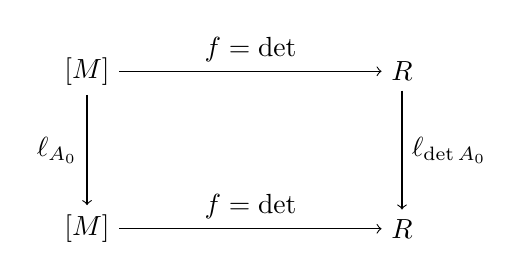
\begin{tikzpicture}
    \node (mani1) at (0, 0) {$\manifold[M]$};
    \node (real1) at (4, 0) {$\mathbb{R}$};
    \node (mani2) at (0, -2) {$\manifold[M]$};
    \node (real2) at (4, -2) {$\mathbb{R}$};
    \draw[->] (mani1) -- (real1) node[midway, above] {$f = \det$};
    \draw[->] (mani2) -- (real2) node[midway, above] {$f = \det$};
    \draw[->] (real1.south) -- (real2.north) node[midway, right] 
        {$\ell_{\det A_0}$};
    \draw[->] (mani1.south) -- (mani2.north) node[midway, left] 
        {$\ell_{A_0}$};
\end{tikzpicture}
        \end{center}
        \par
        So we know
        \[
        f = \ell_{\det A_0}^{-1}\circ f\circ \ell_{A_0}.
        \]
        We know that both \(\ell_{A_0} : A \mapsto A_0A\) and \(\ell_{\det A_0}
        : a \mapsto a \det A_0\) are linear and thus 
        \(C^\infty\) diffeomorphisms. Therefore, 
        \[
        \begin{aligned}
            \rank f_{*A_0} &= \rank (\ell_{\det A_0 ^{-1} }^{-1}\circ 
            f\circ \ell_{A_0 ^{-1}})_{*A_0} \\
            &= \rank (\ell_{\det A_0 ^{-1}}^{-1}\circ f)_{*I} \\
            &= \rank (f_{*I}).
        \end{aligned}
        \]
        Then one can use the elementary argument again, but this time with 
        significantly less complexity.
    \end{proof}
    \begin{theorem}[Dimension of Orthogonal Group \(\ONR{n}\)]\label{thm:dim-onr}
        The orthogonal group \(\ONR{n}=\Set{A \in M_n(\mathbb{R})|AA ^{\top}
        =I_n}\) is a \(C^\infty\) submanifold of \(\GLNR{n}\) of codimension 
        \(\frac{n(n+1)}{2}\), and thus \(\dim \ONR{n}=\frac{n(n-1)}{2}\).
    \end{theorem}
    \begin{proof}
        Consider the following diagram,
        \begin{center}
            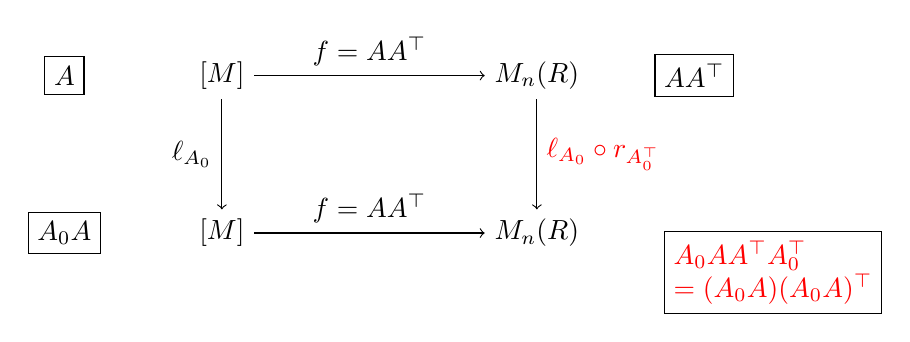
\begin{tikzpicture}
    \node (mani1) at (0, 0) {$\manifold[M]$};
    \node (real1) at (4, 0) {$M_n(\mathbb{R})$};
    \node (mani2) at (0, -2) {$\manifold[M]$};
    \node (real2) at (4, -2) {$M_n(\mathbb{R})$};
    \draw[->] (mani1) -- (real1) node[midway, above] {$f = AA ^{\top}$};
    \draw[->] (mani2) -- (real2) node[midway, above] {$f = AA ^{\top}$};
    \draw[->] (real1.south) -- (real2.north) node[midway, right, text=red] 
        {$\ell_{A_0}\circ r_{A_0 ^{\top}}$};
    \draw[->] (mani1.south) -- (mani2.north) node[midway, left] 
        {$\ell_{A_0}$};
    \node[draw] at (-2, 0) {$A$};
    \node[draw] at (-2, -2) {$A_0A$};
    \node[draw] at (6, 0) {$AA ^{\top}$};
    \node[draw, align=left, text=red] at (7, -2.5) 
    {$A_0AA ^{\top} A_0 ^{\top}$\\$=(A_0A)(A_0A) ^{\top}$};
\end{tikzpicture}
        \end{center}
        where the red words are determined such that the diagram commutes.
    \end{proof}
    \(\)
\end{document}